%stoichiometric

\documentclass[]{beamer}

\mode<presentation>
{ \usetheme{boxes} }

%\usefonttheme[onlylarge]{structurebold}
%\setbeamerfont*{frametitle}{size=\small,series=\bfseries}

\usecolortheme{lily}
\usepackage{multicol}
\usepackage{amsmath}
\usepackage{amsfonts,dsfont}
\usepackage{color}
%\usepackage{graphicx}
\usepackage{listings}

\usepackage{beamerthemesplit}
\usepackage{amssymb}
\usepackage{verbatim}


\usepackage[usenames,dvipsnames]{pstricks}
\usepackage{epsfig}
\usepackage{pst-grad} % For gradients
\usepackage{pst-plot} % For axes
\usepackage{subfig}

\usepackage{wrapfig}
\usepackage{booktabs}
\usepackage{bm}
\usepackage{longtable}

%\usetheme{Warsaw}
% or ...
%\usetheme{Antibes}    % tree outline, neat
%\usetheme{JuanLesPins}    % like Antibes, with shading
%\usetheme{Bergen}    % outline on side
%\usetheme{Luebeck}    % like Warsaw, square sides
%\usetheme{Berkeley}    % interesting left bar outline
%\usetheme{Madrid}    % clean, nice.  7/12 page numbers
%\usetheme{Berlin}    % dots show slide number
%\usetheme{Malmoe}    % OK, plain, unshaded
\usetheme{Boadilla}    % nice, white bg, no top bar
%\usetheme{Marburg}    % nice, outline on right
%\usetheme{boxes}    % ???
%\usetheme{Montpellier}    % tree outline on top, plainish white
%\usetheme{Copenhagen}    % like Warsaw
%\usetheme{PaloAlto}    % looks good
%\usetheme{Darmstadt}    % like Warsaw with circle outline
%\usetheme{Pittsburgh}
%\usetheme{default}
%\usetheme{Rochester}    % like boxy, unshaded warsaw
%\usetheme{Dresden}    % circle outline on top
%\usetheme{Singapore}    % purple gradient top
%\usetheme{Frankfurt}    % like Warsaw with circle outline on top
%\usetheme{Szeged}
%\usetheme{Goettingen}    % light purple right bar outline
%\usetheme{Warsaw}
%\usetheme{Hannover}    % like Goett with bar on left
%\usetheme{compatibility}
%\usetheme{Ilmenau}



%\reversemarginpar
%\topmargin -1.0in
%\oddsidemargin -0in
%\textheight 6in
%\textwidth 8in


%\setbeamertemplate{footline}[page number]


%\usepackage{tikz}
%\usetikzlibrary{arrows}
%\tikzstyle{block}=[draw opacity=0.7,line width=1.4cm]



%\usepackage{}
\def\tcb{\textcolor{blue}}
\def\tcr{\textcolor{red}}
\def\tcg{\textcolor{green}}
\def\mbf{\mathbb{}}
\def\ind{\mathds 1}
\def\BF{BF}

\def\tcr{\textcolor{red}}
\def\tcb{\textcolor{blue}}
\def\ii{{(i)}}
\def\kk{{(k)}}
\def\Theta{\xi}


\def\dir{/Users/yguan/Dropbox/work/2layer/latex/pic/arxiv}
\def\dirb{{/Users/yguan/Dropbox/Shared/quan/selection/pic/}}
\def\hanli{{/Users/yguab/Dropbox/Shared/hanli/}}
\def\dirv{{/Users/yguan/Dropbox/work/vaccine/latex/pic/}}


\def\X{{{X}}}
\def\x{{\bf x}}
\def\y{{\bf y}}
\def\z{{\bf z}}
\def\e{{\bf e}}
\def\a{{\bf a}}
\def\b{{\bf{b}}}
\def\c{{\bf{c}}}
\def\d{{\bf{d}}}
\def\u{{\bf u}}
\def\v{{\bf v}}
\def\q{{\bf q}}
\def\1{{\bf 1}}
\def\g{{\bf g}}
\def\trace{{\text{trace}}}
\def\logbf{{\log_{10}BF}}



\def\e{{\mathbf{\epsilon}}}
\def\u{{\mathbf{u}}}
\def\x{{\mathbf{x}}}
\def\X{{\mathbf{X}}}
\def\g{{\mathbf{g}}}
\def\al{{\mathbf{\alpha}}}
\def\ga{{\mathbf{\gamma}}}
\def\y{{\mathbf{y}}}
\def\bb{{\mathbf{\beta}}}
\def\a{{\mathbf{a}}}
\def\z{{\mathbf{z}}}
\def\Z{{\mathbf{Z}}}
\def\W{{\mathbf{W}}}
\def\Q{{\mathbf{Q}}}
\def\U{{\mathbf{U}}}
\def\D{{\mathbf{D}}}
\def\K{{\mathbf{K}}}
\def\S{{\mathbf{S}}}

\setbeamercovered{dynamic}
% To remove the navigation symbols from
% the bottom of slides%
\setbeamertemplate{navigation symbols}{}
%
\usepackage{graphicx}
%\usepackage{bm}         % For typesetting bold math (not \mathbold)
%\logo{\includegraphics[height=0.6cm]{yourlogo.eps}}
%
%\title[Short title of the talk]{Beautiful Presentation using Beamer}
%\author{Name of the Speaker}
%\institute[U of X]
%{
%University of [...] \\
%\medskip
%{\emph{email@domain.ca}}
%}
%\date{\today}


\title[Kindred]{Estimation of inbreeding and kinship coefficients via latent identity-by-descent states \footnote{This is joint work with Dan Levy.}}
\author{Yongtao Guan} %\\Baylor College of Medicine}
\institute[grant.guan@nih.gov]
{
Framingham Heart Study \\
National Heart, Lung, and Blood Institute  \\ 
\vspace{.2in}
present at \\ Department of Biostatistics, Boston University
}
%\date{\today}
\date{April 21, 2023}


\begin{document}

\frame{\titlepage}

%%%%%%%%%%%%%%%%%%%%%%%%%%%%%%%%%%%%%%%%%%
%\begin{frame}{Self Introduction}
%\begin{itemize}
%\item B.S. Southeast University (Alumni award)  
%\item Ph.D. University of Idaho, Probability and Stochastic processes.  
%\item Postdoc University of Chicago, Bayesian statistics and statistical genetics. 
%\item Assistant Professor, Baylor College of Medicine, Lead a small but intense group.  
%\item Current research interests: haplotype variation and its phenotypic consequences in humans, Bayesian statistics, de novo assembly. 
%\end{itemize}
%\end{frame}
%
%
%
%%%%%%%%%%%%%%%%%%%%%%%%%%%%%%%%%%%%%%%%%%
%\begin{frame}{Self Introduction}
%\begin{center}
%\includegraphics[height=0.95\textheight]{/Users/yongtaog/Dropbox/Photos/me+xcluster.jpg}
%\end{center}
%\end{frame}

\section{Introduction}
%%%%%%%%%%%%%%%%%%%%%%%%%%%%%%%%%%%%%%
\begin{frame}{Kinship and inbreeding coefficients}
\begin{itemize}
\item Kinship (denoted by $\phi$) is the probability that two alleles sampled each from two individuals are identical by descent (IBD).
\item Kinship between two individuals is the inbreeding coefficient (denoted by $F$) of their (hypothetical) children. 
\item Between one and oneself (or between monozygotic twins) $\phi = (1+F)/2$. 
\item Inbreeding can be treated as a derived concept of kinship. 
\end{itemize}
%\vskip0.2cm
%\begin{center}
%\includegraphics[width=0.80\textwidth]{\dir/../cartoon}
%\end{center}
\end{frame}




%%%%%%%%%%%%%%%%%%%%%%%%%%%%%%%%%%%%%%%
\begin{frame}{Identity by descent (IBD)}

The definitions of inbreeding and kinship hinge on IBD, while IBD is defined relative to a reference population, where different alleles in that reference population are considered \emph{not} IBD~\footnote{Wang, J. (2016). Theor. Popul. Biol. 107, 4–13}. 

\end{frame}

%%%%%%%%%%%%%%%%%%%%%%%%%%%%%%%%%%%%%%
\begin{frame}{Existing methods to infer kinship}
 \begin{itemize}
 \item  Sample correlation based genetic relatedness matrix (scGRM).     
 \item  UKin, aims to correct bias observed in scGRM methods~\footnote{Jiang, W., et. al, and H. Zhao (2022). BMC Bioinformatics 23(1), 525}. 
 \item  King, based on counts of a subset of joint genotypes~\footnote{Manichaikul, A, and et. al, and W.-M. Chen (2010). Bioinformatics 26(22), 2867– 2873.}
 \end{itemize}
 All three produced substantial amount of negative estimates for kinship, difficult to interpret. 
\end{frame}

\section{Results}
%%%%%%%%%%%%%%%%%%%%%%%%%%%%%%%%%%%%%%%
\begin{frame}{Jacquard IBD states} 
\begin{center} 
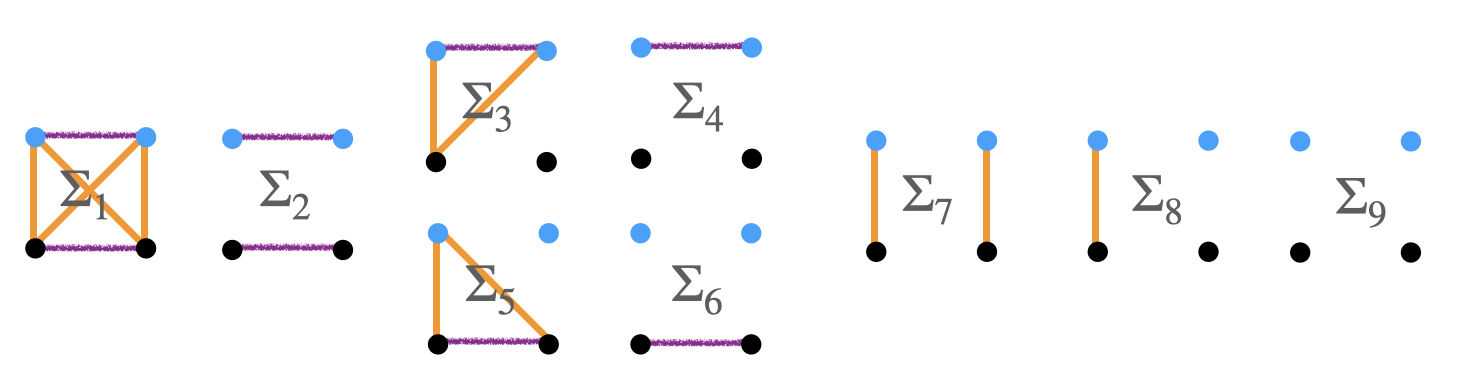
\includegraphics[width=0.8\textwidth]{jacquard.png}  
\end{center}
%\vspace{.1in}
Kinship can be computed from the loading probabilities, $\Delta_j$ for $j$-th latent IBD state $\Sigma_j$, as follows~\footnote{Jacquard, A. (1972). Biometrics 28(4), 1101–1114.} 
\begin{equation}\label{e1}
\begin{aligned}
\phi &= \Delta_1 + \frac{1}{2}(\Delta_3+\Delta_5+\Delta_7) + \frac{1}{4} \Delta_8.  \\
\end{aligned}
\end{equation}
Inbreeding coefficients can also be computed: 
\begin{equation}\label{e2}
\begin{aligned}
F_1 &= \Delta_1 + \Delta_2 + \Delta_3 + \Delta_4, \\                                                                                                     
F_2 &= \Delta_1 + \Delta_2 + \Delta_5 + \Delta_6. \\
\end{aligned}
\end{equation}


\end{frame}


%%%%%%%%%%%%%%%%%%%%%%%%%%%%%%%%%%%%%%%
\begin{frame}{Jacquard IBD states} 
Each latent IBD states emit joint genotypes at a probability distribution that is a function of allele frequency $p.$~\footnote{Thompson, E. A. (2013).  Genetics 194(2), 301–326.}
\begin{center} 
\begin{tabular}{lllllllll|ll}
 $\Sigma_1$ &  $\Sigma_2$ &  $\Sigma_3$ &  $\Sigma_4$ &  $\Sigma_5$ &  $\Sigma_6$ &  $\Sigma_7$ &  $\Sigma_8$ &  $\Sigma_9$ &G1 & G2 \\
\hline 
 $p$ & $p^2$ & $p^2$ & $p^3$ & $p^2$ & $p^3$ & $p^2$ & $p^3$ & $p^4$ & AA &AA \\       
 $0$ & $0$ & $pq$ & $2p^2q$ & $0$ & $0$ & $0$ & $p^2q$ &$2p^3q$ &AA &AB  \\
 $0$ & $pq$ & $0$ & $pq^2$ & $0$ & $p^2q$ & $0$ & $0$ &$p^2q^2$ &AA &BB \\
 $0$ & $0$ & $0$ & $0$ & $pq$ & $2p^2q$ & $0$ & $p^2q$ &$2p^3q$ & AB &AA   \\
$0$ & $0$ & $0$ & $0$ & $0$ & $0$ & $2pq$ & $pq$ &$4p^2q^2$ & AB &AB   \\
 $0$ & $0$ & $0$ & $0$ & $pq$ & $2pq^2$ & $0$ & $pq^2$ &$2pq^3$ & AB &BB \\
$0$ & $pq$ & $0$ & $p^2q$ & $0$ & $pq^2$ & $0$ & $0$ &$p^2q^2$ & BB &AA   \\
 $0$ & $0$ & $pq$ & $2pq^2$ & $0$ & $0$ & $0$ & $pq^2$ &$2pq^3$ &BB &AB   \\
 $q$ & $q^2$ & $q^2$ & $q^3$ & $q^2$ & $q^3$ & $q^2$ & $q^3$ & $q^4$ &BB &BB \\       
  \end{tabular} 
  \end{center}
  where $q = 1-p.$ Our aim is to infer $\Delta_j$, the loading probabilities of $\Sigma_j$. 
\end{frame}


%%%%%%%%%%%%%%%%%%%%%%%%%%%%%%%%%%%%%%%%%%%%
\begin{frame}{Fit the model}
We consider SNPs with allele frequency $p$ so that they share the same $\Sigma$ matrix.  Denote $\hat\theta$ estimates of fractions of joint genotypes (AA AA, AA AB, ... etc).   
\begin{subequations} \label{lse}
\begin{align}
{\text{arg} \min_\Delta\;\;}  &||\S_p \Delta - \hat\theta_p ||_2  \label{eq:lse} \\
       \mbox{s.t \;\;} \Delta_j & \ge 0  \mbox{\;\;for all $j$, \;and} \sum \Delta_j  = 1 \label{eq:st}
\end{align}
\end{subequations}
where $\S_p = (\Sigma_1, \dots, \Sigma_9)$, $\Delta=(\Delta_1, \dots, \Delta_9)$ is the vector of loading probabilities. 

\end{frame}

%%%%%%%%%%%%%%%%%%%%%%%%%%%%%%%%%%%%%%%%%%%%
\begin{frame}{Fit the model}
For the $i$-th SNP with allele frequency $p_i$, we can compute $\S_{p_i}$ and we observe $\hat{\theta}=e_i$, where $e_i$ has a single entry $1$ and the rest $8$ entries $0$.  %We append $\S_{p_i}$'s together to obtain the design matrix $\S$ and append $e_i$'s together to obtain a vector $\hat\theta$. For total $m$ SNPs, $\S$ is an $9m \times 9$ matrix, and $\hat\theta$ is an $9m$ vector, and we seek the least square fit of a constrained system
\begin{equation} \label{lse2}
%\begin{aligned}
{\text{arg} \min_\Delta\;\;}  ||\S \Delta - \hat\theta ||_2  %\\
   %    \mbox{s.t \;\;} \Delta_j & \ge 0  \mbox{\;\;for all $j$, \;and} \sum \Delta_j  = 1. 
%\end{aligned}
\end{equation}
with constraints \eqref{eq:st}. The above system generalizes \eqref{lse} to SNPs of arbitrary allele frequencies.  In practice, we find binning SNPs and re-estimate allele frequencies in each bin improves performance. 

\end{frame}



%%%%%%%%%%%%%%%%%%%%%%%%%%%%%%%%%%%%%%%%%%%%
\begin{frame}{Fit the model: invariant}
It can be verified that there are two linear dependence in $\S_p$. One is  $\Sigma_2 + 2 \Sigma_8 = \Sigma_4 + \Sigma_6 + \Sigma_7$ and the other is $pq (\Sigma_1+\Sigma_2- 2\Sigma_3 - 2\Sigma_5 + 2\Sigma_7)  =  \Sigma_7 - 2 \Sigma_8 +  \Sigma_9$. Therefore, the solution to the system $\S \Delta = \hat\theta$ is not unique. Let $\S^{+}$ be Moore-Penrose inverse of $\S$, then $\Delta = \S^{+} \hat\theta + (I - \S^{+} \S) v$ for any vector $v$.  Denote $C = (I - \S^{+} \S) v$,  it can be verified that  
\begin{equation}\label{C}
\begin{aligned}
C_1 =C_3=C_5=C_9 &= 0 \\
C_2  &=  \frac{1}{8} v_2 -  \frac{1}{8} v_4 -  \frac{1}{8} v_6 -  \frac{1}{8} v_7 +  \frac{1}{4} v_8 \\  
C_4 =  C_6 = C_7 &=  - \frac{1}{8} v_2 +  \frac{1}{8} v_4 +  \frac{1}{8} v_6 +  \frac{1}{8} v_7 -  \frac{1}{4} v_8 \\
%C_6 &= - \frac{1}{8} v_2 +  \frac{1}{8} v_4 +  \frac{1}{8} v_6 +  \frac{1}{8} v_7 -  \frac{1}{4} v_8 \\
% C_7 &=   - \frac{1}{8} v_2 +  \frac{1}{8} v_4 +  \frac{1}{8} v_6 +  \frac{1}{8} v_7 -  \frac{1}{4} v_8 \\
  C_8 &= \frac{1}{4} v_2 - \frac{1}{4}  v_4 - \frac{1}{4}  v_6 - \frac{1}{4}  v_7 + \frac{1}{2}  v_8. \\
\end{aligned}
\end{equation}
1)  $\Delta_1, \Delta_3, \Delta_5$, and $\Delta_9$ are not affected by $v$ and these components have unique solutions. 2) $C_2 + C_4 = 0$, $C_2+C_6 = 0$ and $C_7 + \frac{1}{2}C_8 = 0$, which means,  $\Delta_2+\Delta_4 $, $\Delta_2+\Delta_6$, and  $\Delta_7 + \frac{1}{2}\Delta_8$ are invariant. 3) Consequently $\phi$ in Equation~\eqref{e1} and $F_1$ and $F_2$ in Equation~\eqref{e2} are unique. 
\end{frame}


%%%%%%%%%%%%%%%%%%%%%%%%%%%%%%%%%%%%%%%%%%%%
\begin{frame}{Simulated non-admixed samples}
\begin{center}
\includegraphics[width=0.9\textwidth,height=0.68\textwidth]{comp2-tall.pdf}
\end{center}
\end{frame}

%%%%%%%%%%%%%%%%%%%%%%%%%%%%%%%%%%%%%%%%%%%%
\begin{frame}{Comparisons between with and without inbreeding}
\begin{center}
\includegraphics[width=0.9\textwidth,height=0.68\textwidth]{comp-j9j3.pdf}
\end{center}
%{Not modeling inbreeding bias kinship estimates. Gray colors are results from using all nine latent IBD states (with inbreeding); Plum colors are results from using the last three latent IBD states (without inbreeding). Due to the scale of the plot on y-axis, the biases are more visible between more distant relatedness.}
\end{frame}


%%%%%%%%%%%%%%%%%%%%%%%%%%%%%%%%%%%%%%%%%%%%
%\begin{frame}{Using SNPs of small population divergence to mimic ancestral allele frequencies}
%\begin{itemize}
%\item obtained all bi-allelic SNPs with minimum count of minor alleles 50 (among 2504 samples). 
%\item counted AN-AC for different populations.  
%\item did a chisq test for each SNP to obtain a p-values, with null hypothesis as equal allele frequency across three populations.  
%\item wrote a vcf file with allele frequencies and an additional tag INFO/FST = -10log10(p-value).  
%\item SNPs whose $FST < 3$ appears to be working well for admixed samples, and there are about $1.2$ million such bi-allelic SNPs in 1000 genomes.   
%\end{itemize}
%\end{frame}

\begin{frame}{Kinship between admixed samples}
\begin{itemize}
%If the continental population were taken as the homogenous reference population for IBD for non-admixed samples, then for admixed samples 
\item The reference population for IBD for admixed samples has to be the ancestral population predates continental population divergence. 
\item This ancestral population can be partially mimicked by selecting a set of SNPs  whose allele frequencies are similar across different continental populations. 
\item Among 12 million bi-allelic SNPs with minimum 50 minor allele counts (out of total 2504 diplotypes) in 1000 genomes project, there are $1.2$ million such SNPs.  
\item We also randomly selected common bi-allelic SNPs of $1.2$ million,  and used these to compute kinship for comparison. 
\end{itemize}
\end{frame}

%%%%%%%%%%%%%%%%%%%%%%%%%%%%%%%%%%%%%%%%%%%%
\begin{frame}{Simulated admixed samples}
\begin{center}
\includegraphics[width=0.9\textwidth,height=0.68\textwidth]{admix-sanguo2.pdf}
\end{center}
\end{frame}


%%%%%%%%%%%%%%%%%%%%%%%%%%%%%%%%%%%%%%%%%%%%
\begin{frame}{1000 genomes samples}
\begin{center}
\includegraphics[width=0.6\textwidth]{1000g-pop7.pdf}
\end{center}
\end{frame}


\begin{frame}{random common vs small population divergence SNPs}
\begin{center}
\includegraphics[width=0.65\textwidth]{pairs2.png}\\
\vspace{-0.05in}
{\tiny Africans (in black), Americans (in red), East Asians (in green), Europeans (in blue), and South asians (in cyan).}
\end{center}
\end{frame}

%%%%%%%%%%%%%%%%%%%%%%%%%%%%%%%%%%%%%%
\begin{frame}{Chr17: Asian vs African freq. (Kindred), and scGRM.}
\begin{center}
\includegraphics[width=0.49\textwidth]{pairs-chr17.png}
\includegraphics[width=0.49\textwidth]{pairs-chr17-rel.png}\\
\includegraphics[width=0.2425\textwidth]{pairs-chr17-ph.png} 
\includegraphics[width=0.2425\textwidth]{pairs-chr17-bf.png} 
\includegraphics[width=0.2425\textwidth]{pairs-chr17-rel-ph.png} 
\includegraphics[width=0.2425\textwidth]{pairs-chr17-rel-bf.png}
\end{center}

\end{frame}


%%%%%%%%%%%%%%%%%%%%%%%%%%%%%%%%%%%%%%%%%%%%
\begin{frame}{Genomic control}
\begin{center}
\begin{tabular}{lccccccccc}
{$\lambda$} &  {None} &  {scGRM}& {UKin} & {King}    & {Kindred} \\ 
 \hline
BD &   1.115  & 0.988 & 0.993 & 1.024   & 1.014 \\
CAD   & 1.078  & 0.985 & 0.993 & 1.019  &1.014 \\
CD   & 1.079   & 0.999 & 1.003 & 1.015  &1.019 \\
HT   & 1.063  & 0.997 & 1.004 & 1.016  &1.014  \\
 RA  & 1.053   & 0.974 & 0.980& 1.000  & 0.989 \\
T1D   & 1.067   & 0.940 & 0.950 & 0.966  &0.972 \\
T2D \footnote{Wellcome Trust Case Control Consortium (2007). Nature 447, 661–678.}    & 1.076   & 0.986 & 0.995 &1.024 &1.008  \\
Height \footnote{Yang, J., et. al. and P. M. Visscher (2010). Nat Genet 42 (7), 565–569.
}   & 1.029   & 0.992 & 0.990 &0.993  & 0.995  \\
\hline
Mean & 1.070& 0.983 & 0.989 & 1.007 & 1.003 \\
SSD & 0.024& 0.019 &  0.017 &  0.020 & 0.016 \\
  \end{tabular}
  \end{center}
\end{frame}
%
%
%
%
%%%%%%%%%%%%%%%%%%%%%%%%%%%%%%%%%%%%%
\begin{frame}{Heritability of height}

{\small
\begin{center}
\begin{tabular}{lccccccc}
   &  {scGRM}& {UKin} & {King}    & {Kindred} \\ 
   \hline
GCTA   &0.449 $\pm$ 0.084 & 0.436 $\pm$ 0.078 &0.376 $\pm$ 0.072 &0.474 $\pm$ 0.085 \\
Gemma\footnote{Zhou, X. and M. Stephens (2012). Nat Genet 44(7), 821–824} &0.446 $\pm$ 0.084 & 0.426 $\pm$ 0.079 & 0.393 $\pm$ 0.071 &0.473 $\pm$ 0.085  \\
\hline
%90\% & 0.455 $\pm$ 0.045 &0.445 $\pm$ 0.038 &0.410 $\pm 0.032$ &0.486 $\pm$ 0.041\\
%70\% & 0.448 $\pm$ 0.086 &0.470 $\pm$ 0.086 &0.406 $\pm 0.078$ &0.500 $\pm$ 0.088\\
%50\% & 0.477 $\pm$ 0.151 &0.486 $\pm$ 0.111 &0.395 $\pm 0.126$ &0.533 $\pm$ 0.160\\
%\hline
\end{tabular}
\end{center}
 %Top two rows entries are PVE $\pm$ se estimated from a single dataset of $3925$ samples; Bottom three rows the entries are mean $\pm$ se of 100 independent trials, in each trial PVE was estimated using our Bayesian MAP estimates.
%  In the three resampling studies, 90\%, 70\% and 50\% of the $3925$ samples were sampled without replacement in each trial. 
We tried to do down-sampling study, but GCTA produced nonsensical results. 

}
\end{frame}



%%%%%%%%%%%%%%%%%%%%%%%%%%%%%%%%%%%%%%
\begin{frame}{MAP estimates for heritability}
Consider a linear model 
\begin{equation} \label{M1}
\begin{aligned}
M0: \y &= \W \alpha  + \e \\
\alpha &\sim MVN(0,  \tau^{-1}  V_W) \\
%\u &\sim MVN_m(0, \eta \tau^{-1} K) \\
\e &\sim MVN_n(0, \tau^{-1} I_n).
\end{aligned}
\end{equation}
%where $\W$ is a $n\times w$ representing $w$ nuisance covariates.    
Adding a random effect $\u$ we have a new model 
%
\begin{equation} \label{M2Z}
\begin{aligned}
M1: \y &= \W \alpha  + \Z \u + \e \\
%\alpha &\sim MVN(0, \tau^{-1} V_0) \\
\u &\sim MVN_m(0, \tau^{-1} \eta K) \\
%\e &\sim MVN_n(0, \tau^{-1} I_n)
\end{aligned}
\end{equation}
%where $Z$ is $n \times m$ matrix presenting the loading, and $K$ is $m\times m$ covariance matrix.   
Let $Q$ and $D$ be eigen decomposition such that $ZKZ^t=QDQ^t$, we have %,   where $D=diag(d_1, \dots, d_n)$ with $d_1 \ge d_2 \ge \dots \ge d_n$ and $QQ^t = I$.  
% Equations~\ref{M2Z} can be rewritten as 
\begin{equation} \label{M2}
\begin{aligned}
M2: \y &= \W \alpha  + Q \ga + \e \\
%\alpha &\sim MVN(0, \tau^{-1} V_0) \\
\ga &\sim MVN_n(0, \tau^{-1} V_Q) \\
%\e &\sim MVN_n(0, \tau^{-1} I_n)
\end{aligned}
\end{equation}
where $V_Q = \eta D$. To see this, $$E(Z\u\u^tZ^t) = \eta ZKZ^t = \eta QDQ^t = E(Q\gamma \gamma^t Q^t).$$ 
\end{frame}



\begin{frame}{MAP estimates for heritability}

{\small
Denote $X = (Q, W)$ and $V = \left( \begin{smallmatrix} \eta D & 0 \\  0 & V_W \end{smallmatrix} \right),$ using normal inverse gamma prior to get 
\begin{equation}
BF(\eta) = \frac{\det(W^tW)^{1/2} }{\det(\X^t \X + V^{-1})^{1/2} \det(V_Q)^{1/2}} \left( \frac{\y^t \y - \y^t \X (\X^t \X + V^{-1})^{-1} \X^t \y} {\y^t\y-\y^t W (W^t W)^{-1} W^t \y}   \right)^{-n/2} 
\end{equation}
Bayes factor can be evaluated efficiently for different $\eta$. 

$$\det(X^tX + V^{-1}) = \det(I_n+\frac{1}{\eta D}) \det(W^tW - W^t Q (I_n +\frac{1}{\eta D})^{-1} Q^t W);$$

Denote $F=(I_n+\frac{1}{\eta D})^{-1}$, $M = (W^tW - W^t Q F Q^t W)^{-1}$ to get 
%
$$(X^tX + V^{-1})^{-1} = \left( \begin{smallmatrix} F+F Q^t W M W^t Q F & -F Q^t W M \\ -M W^t Q F& M \end{smallmatrix} \right). $$
We can use Nelder-Mead method to optimize $BF(\eta)$ over $\eta$. 

}
\end{frame}


%%%%%%%%%%%%%%%%%%%%%%%%%%%%%%%%%%%%%%
\begin{frame}{Simulations heritability $30\%$}
\begin{center}
\includegraphics[width=0.48\textwidth]{h30.pdf}
\includegraphics[width=0.48\textwidth]{h30-vp.pdf}
\end{center}
\end{frame}


\begin{frame}{Heritability of height: down sampling study}

{\small
\begin{center}
\begin{tabular}{lccccccc}
   &  {scGRM}& {UKin} & {King}    & {Kindred} \\ 
%   \hline
%GCTA   &0.449 $\pm$ 0.084 & 0.436 $\pm$ 0.078 &0.376 $\pm$ 0.072 &0.474 $\pm$ 0.085 \\
%Gemma &0.446 $\pm$ 0.084 & 0.426 $\pm$ 0.079 & 0.393 $\pm$ 0.071 &0.473 $\pm$ 0.085  \\
\hline
90\% & 0.455 $\pm$ 0.045 &0.445 $\pm$ 0.038 &0.410 $\pm 0.032$ &0.486 $\pm$ 0.041\\
70\% & 0.448 $\pm$ 0.086 &0.470 $\pm$ 0.086 &0.406 $\pm 0.078$ &0.500 $\pm$ 0.088\\
50\% & 0.477 $\pm$ 0.151 &0.486 $\pm$ 0.111 &0.395 $\pm 0.126$ &0.533 $\pm$ 0.160\\
\hline
\end{tabular}
\end{center}
% Top two rows entries are PVE $\pm$ se estimated from a single dataset of $3925$ samples; Bottom three rows the entries are mean $\pm$ se of 100 independent trials, in each trial PVE was estimated using our Bayesian MAP estimates.
%  In the three resampling studies, 90\%, 70\% and 50\% of the $3925$ samples were sampled without replacement in each trial. 
}
\end{frame}




%%%%%%%%%%%%%%%%%%%%%%%%%%%%%%%%%%%%%%
\begin{frame}{Summary}
\begin{itemize}
\item Kindred use non-negative least square to compute loadings of latent IBD states to infer kinship and inbreeding coefficients. 
\item Kindred allows one to specify reference populations (through specifying the set of allele frequencies). 
\item By choosing a set of small population divergence SNPs, kindred is also effective for admixed samples. 
\item Kindred is effective to control for population structure and relatedness in GWAS. 
\item Kindred produces slightly large but statistically significant estimates on heritability. 
\item Software is available at \url{www.haplotype.org}. 
\end{itemize}

\end{frame}

%%%%%%%%%%%%%%%%%%%%%%%%%%%%%%%%%%%%%%%
%\begin{frame}{Phasing problem in 1000G}
%\begin{center}
%\includegraphics[width=12cm]{\dir/../unphased-phased.pdf}
%\end{center}
%\end{frame}


%%%%%%%%%%%%%%%%%%%%%%%%%%%%%%%%%%%%%%%
%\begin{frame}{Summary of local ancestry inference}
%\begin{itemize}
%\item Cleanly handle multi-way admixture.
%\item Cleanly handle missing data. 
%\item Does not require phased ancestry reference populations.
%\item Does not require known genetic map.  
%\item Does not require to label the reference populations.   
%\item Can average over multiple choices of $\gamma$, the admixture generations, to relax the assumption of the single-pulse admixture. 
%%\item Time since admixing events happened can be estimated. 
%%%\item It takes similar amount of time as to perform imputation.
%%\item MALD (mapping via Admixture LD) and case-only design.
%\end{itemize}
%\end{frame}
%

%%%%%%%%%%%%%%%%%%%%%%%%%%%%%%%%%%%%%%%
%\begin{frame}{Local ancestry of Mexicans}
%\begin{center}
%\includegraphics[width=8cm]{\dir/../mex-concordance2.pdf}
%\end{center}
%\end{frame}


%%%%%%%%%%%%%%%%%%%%%%%%%%%%%%%%%%%%%%%
%\begin{frame}{Local ancestry of Mexicans}
%\begin{center}
%\includegraphics[width=12cm]{\dir/../local-enrich-chr6.pdf}
%\end{center}
%\end{frame}
%
%%%%%%%%%%%%%%%%%%%%%%%%%%%%%%%%%%%%%%%%
%%\begin{frame}{Local ancestry of Mexicans}
%%\begin{center}
%%\includegraphics[width=12cm]{\dir/../local-enrich-chr8.pdf}
%%\end{center}
%%\end{frame}
%
%%%%%%%%%%%%%%%%%%%%%%%%%%%%%%%%%%%%%%%%
%%\begin{frame}{Local ancestry of Puerto Ricans}
%%
%%\begin{center}
%%\includegraphics[width=5cm]{\dir/../tang.jpeg}
%%\end{center}
%%
%%\footnotesize{Tang etal. (AJHG, 2007) identified three regions under strong selection.  
%%Price etal (AJHG 2008) argued that 1) long range LD can be a problem; 2) inaccurate reference; 3) failed to replicate using ANCESTRYMAP on a larger, 364 Puerto Rican samples.}
%%\end{frame}
%%
%%
%%
%%%%%%%%%%%%%%%%%%%%%%%%%%%%%%%%%%%%%%%%
%%\begin{frame}{No selection in African Americans}
%%
%%\begin{center}
%%\includegraphics[width=10cm]{\dirb/aa-nosel.png}
%%\end{center}
%%
%%\footnotesize{In an effort to generalize their null claim, they questioned the chr6 Mexican selection signal reported in ELAI paper. Their arguments: 1) too strong to be true; 2) not found by other methods, namely, HAPMIX, LAMP-LD, RFMix, and MultiMix.}
%%\end{frame}
%%
%
%%%%%%%%%%%%%%%%%%%%%%%%%%%%%%%%%%%%%%%
%\begin{frame}{Global ancestry of Mexicans in two GWAS data sets}
%%1. Viva la Familia  study contains $815$ individuals in nuclear families. 
%
%\begin{center}
%%\includegraphics[width=6cm]{\dirb/viva-5panel-all-admix-tri.pdf} 
%%\includegraphics[width=6cm]{\dirb/viva-pca2.pdf}
%%%\includegraphics[width=5cm]{\dir/../viva-admix.png}
%
%\includegraphics[width=4cm]{\dirb/viva-5panel-all-admix-tri.pdf} 
%\includegraphics[width=4cm]{\dirb/mex-admix-tri.pdf} \\
%\includegraphics[width=4cm]{\dirb/viva-pca2.pdf} 
%\includegraphics[width=4cm]{\dirb/mex-pca2.pdf} 
%
%
%\end{center}
%
%\end{frame}



%%%%%%%%%%%%%%%%%%%%%%%%%%%%%%%%%%%%%%%
%\begin{frame}{Local ancestry of Mexicans in two GWAS data sets}
%%1. Viva la Familia  study contains $815$ individuals in nuclear families. 
%2. Mexican lipid  study contains $2229$ unrelated individuals.  
%
%\begin{center}
%\includegraphics[width=6cm]{\dirb/mexican0-admix-tri.pdf}
%\includegraphics[width=6cm]{\dirb/mexctrl-pca2.pdf} 
%
%%\includegraphics[width=5cm]{\dir/../viva-admix.png}
%
%\end{center}
%
%\end{frame}

%%%%%%%%%%%%%%%%%%%%%%%%%%%%%%%%%%%%%%
%\begin{frame}{Local ancestry of Mexicans in two GWAS data sets}
%1. Viva la Familia  study contains $815$ individuals in nuclear families. 
%2. Mexican lipid  study contains $2229$ unrelated individuals.  
%
%\begin{center}
%%\includegraphics[width=6cm]{\dirb/viva-ceu-yri-maya-all-combined.png}
%%\includegraphics[width=6cm]{\dirb/mexican-ceu-yri-maya-all-combined.png}
%\includegraphics[width=6cm]{\dirb/viva-ceu-yri-maya-all-african.png}
%\includegraphics[width=6cm]{\dirb/mexican-ceu-yri-maya-all-african.png}
%
%%\includegraphics[width=5cm]{\dir/../viva-admix.png}
%
%\end{center}
%
%\end{frame}
%
%
%%%%%%%%%%%%%%%%%%%%%%%%%%%%%%%%%%%%%%%
%\begin{frame}{MHC}
%\begin{center}
%\vspace{-1cm}
%\includegraphics[width=8cm]{\dirb/mexican-compare-references.png} \\
%%\includegraphics[width=5cm]{\dirb/mexican-compare-references1.png} \\
%\includegraphics[width=5cm]{\dirb/mexican-diff1.pdf}\footnote{B*15:01, B*07:02, C*04:01}
%\includegraphics[width=5cm]{\dirb/structure-hapmap3.pdf}
%
%\end{center}
%\end{frame}
%

%%%%%%%%%%%%%%%%%%%%%%%%%%%%%%%%%%%%%%%
%\begin{frame}{Local ancestry of Mexicans in two GWAS data sets}
%1. Viva la Familia  study contains $815$ individuals in nuclear families. 
%2. Mexican lipid  study contains $2229$ unrelated individuals.  
%
%\begin{center}
%\includegraphics[width=6cm]{\dirb/viva-american.png}
%\includegraphics[width=6cm]{\dirb/mexican-ctrl-american.png} 
%
%%\includegraphics[width=5cm]{\dir/../viva-admix.png}
%
%\end{center}
%
%\end{frame}

%%%%%%%%%%%%%%%%%%%%%%%%%%%%%%%%%%%%%%%
%\begin{frame}{Local ancestry of Mexicans in two GWAS data sets}
%\begin{itemize}
%\item Long-range LD 
%\item Inaccurate reference panels.
%%\item Not discovered by other methods.   
%\end{itemize}
%\begin{center}
%%\includegraphics[width=6cm]{\dirb/mexican-chr6-2panel-s20.png}
%\includegraphics[width=6cm]{\dirb/viva-chr6-2panel-afr.png}
%\includegraphics[width=6cm]{\dirb/mexican-chr6-2panel-afr.png}
%
%\end{center}
%
%
%\end{frame}
%
%
%
%%%%%%%%%%%%%%%%%%%%%%%%%%%%%%%%%%%%%%%
%\begin{frame}{Local ancestry of Mexicans in two GWAS data sets}
%\begin{itemize}
%\item Strong selection.  $0.05 \times (1+ s)^{20} = 0.2$ to get $s=0.07$. 
%\item What drives it? some pathogen? 
%\item Some artifacts? but we are careful. We removed all A/T, C/G SNPs. We redid the inference without the Maya+Pima samples and signal remains. We remove SNPs whose cluster plots is not ``normal." 
%\item  An epidemic, called ``Huey Cocoliztli," was symptomatically different from those imported from the Old World, began in 1545, and lingered around until 1815. The epidemic, which some medical historians suspected a haemorrhagic fever caused by arenavirus carried by rodents,  selectively targets native people, and 90\% of population perished in a few generations. 
%\end{itemize}
%\end{frame}
%
%
%%%%%%%%%%%%%%%%%%%%%%%%%%%%%%%%%%%%%%%
%\begin{frame}{Local ancestry of Mexicans and Lipid trait}
%\includegraphics[width=12cm]{\dirb/apoa5-chr11.png}
%\end{frame}

%%%%%%%%%%%%%%%%%%%%%%%%%%%%%%%%%%%%%%
%
%\begin{frame}{A linear algorithm for model fitting}
%
%Let $Z_m^1=(X_m^1,Y_m^1)$ and $Z_m^2=(X_m^2,Y_m^2)$ be two sets of latent states at marker $m$ to indicate the upper- and lower-layer cluster for individual $i$. 
%%
%Note each individual has its own set of latent states $(Z_\cdot^1,Z_\cdot^2)$, and we drop the superscript $i$ for simplicity. 
%We are interested in computing the posterior of the latent states
%\begin{equation}\label{eqn:joint}
%\begin{aligned}
%p\left(Z_\cdot^1, Z_\cdot^2 |G, \xi \right) 
%%&= \frac{1}{p(G|\xi)} p(G| \theta_{Z^1}, \theta_{Z^2}, \xi) p(Z^1, Z^2 | \xi) \\
%                                        &= \frac{1}{p(G|\xi)} p(G| \theta_{Z_\cdot^1}, \theta_{Z_\cdot^2}, \xi) p(Z_\cdot^1| \xi) p(Z_\cdot^2| \xi) 
%%&= \Pi_{m=1}^M p(G_m|Z_m^1, Z_m^2, \xi) \Pi_{m=2}^M p(Z_m^1|Z_{m-1}^1, \xi) p(Z_0^1| \xi)  \Pi_{m=2}^M p(Z_m^2|Z_{m-1}^2, \xi) p(Z_0^2| \xi)
%\end{aligned}
%\end{equation}
%where $G=g_{1\dots L}^\ii$, $Z_\cdot^1 = Z_{1\dots L}^1$ and $Z_\cdot^2 = Z_{1\dots L}^2$. 
%First marginalize over $Z_\cdot^2$, and we obtain
%\begin{equation}\label{eqn:marz2}
%\begin{aligned}
%p\left(Z_\cdot^1 |G, \xi \right) %&= \frac{1}{p(G|\xi)} \sum_{Z_m^2} {p(G| \theta_{Z_m^1}, \theta_{Z_m^2}, \xi) p(Z_m^1| \xi) p(Z_m^2| \xi)} \\
%                                         &=\frac{1}{p(G|\xi)} \Pi_{m=1}^M p(G_m|\theta_{Z_m^1}, E_{Z_m^2|\xi}(\theta_{Z_m^2}), \xi) p(Z_m^1| \xi). 
%%&= \Pi_{m=1}^M p(G_m|Z_m^1, Z_m^2, \xi) \Pi_{m=2}^M p(Z_m^1|Z_{m-1}^1, \xi) p(Z_0^1| \xi)  \Pi_{m=2}^M p(Z_m^2|Z_{m-1}^2, \xi) p(Z_0^2| \xi)
%\end{aligned}
%\end{equation}
%Denote $t_m^2 = E_{Z_m^2|\xi}(\theta_{Z_m^2})$,
%we may compute forward and backward probabilities from the marginalization to get $p(Z_m^1|G, \xi)$ for all $m$, and obtain 
%$t_m^1 = E_{Z^1|t_\cdot^2,\xi}(\theta_{Z_m^1})$. 
%\end{frame}
%
%\begin{frame}{A linear algorithm for model fitting}
%
%Then marginalize over $Z_\cdot^1$ to compute conditional probability of $Z_\cdot^2$, where $\theta_{Z_m^1}$ is substituted by $t_\cdot^1$ (the approximation step).  We have
%\begin{equation}\label{eqn:marz1}
%\begin{aligned}
%p\left(Z_\cdot^2 |G, t_\cdot^1, \xi \right) %&= \frac{1}{p(G|t^1, \xi)} \sum_{Z^2} {p(G| \theta_{Z^1}, \theta_{Z^2}, \xi) p(Z^1| \xi) p(Z^2| \xi)} \\
%                                         =\frac{1}{p(G|t_\cdot^1, \xi)} \Pi_{m=1}^M p(G_m|t_m^1, \theta_{Z_m^2}, \xi) p(Z_\cdot^2|\xi). 
%\end{aligned}
%\end{equation}
%%
%In words, we first marginalize over $Z_\cdot^2$ under the prior distribution $p(Z_\cdot^2|\xi)$, 
%and then we make a prediction of allele frequencies $t_\cdot^1$ at each loci based on the marginal posterior distribution of $Z_\cdot^1$. Then conditional on the $t_\cdot^1$
%we compute marginal posterior distribution of $Z_\cdot^2$ (and additionally can obtain updated $t_\cdot^2$). 
%The joint posterior is approximated by two marginals in the sense that for any linear function $f(\theta_{z_1},\theta_{z_2})$, we have
%\begin{equation} \label{eqn:z1z2}
%\begin{aligned}
%E_{Z_\cdot^1,Z_\cdot^2|G,\xi} f(\theta_{z_1},\theta_{z_2}) \approx  E_{Z_\cdot^1|G,t_\cdot^2, \xi} f(\theta_{z_1}, t_{\cdot}^2) + E_{Z_\cdot^2|G,t_\cdot^1, \xi} f(t_{\cdot}^1, \theta_{z_2}). 
%  %    p(Z^1, Z^2 |G, \xi) \approx p(Z_1|G, t_\cdot^2, \xi) p(Z_2|G, t_\cdot^1, \xi). 
%\end{aligned}
%\end{equation}
%%
%The marginal forward and backward probabilities are similar to the forward and backward probabilities of a haploid individual;  We call this algorithm \emph{stochastic linear iterative marginalization}.
%\end{frame}
%%%%%%%%%%%%%%%%%%%%%%%%%%%%%%%%%%%%%%%
%
%\begin{frame}{Performance of the linear algorithm}
%Define local haplotype sharing (LHS) at each marker between two individuals as the inner product of the loading of the lower-layer clusters.  
%\begin{center}
%\includegraphics[width=6cm]{\dir/../lhs-quadratic-linear.pdf}
%\includegraphics[width=6cm]{\dir/../lhs.pdf}
%\end{center}
%\end{frame}
%
%%%%%%%%%%%%%%%%%%%%%%%%%%%%%%%%%%%%%%%%%
%%\begin{frame}{Extending to nuclear family}
%%\begin{itemize}
%%\item Conditional on parental latent states, children are independent. 
%%\item This allows us to write the joint distribution of the latent states for a nuclear family. 
%%\item Children's latent state space is binary, which helps with the computation. 
%%\item Intuitively, the linear algorithm can be worked out. 
%%\end{itemize}
%%\end{frame}
%%

%
%%%%%%%%%%%%%%%%%%%%%%%%%%%%%%%%%%%%%%
%\begin{frame}{Haplotype association}
%Assume a random matrix $M$, of $n\times d$, follows a matrix normal \footnote{Minka, unpulished manuscript, 1996 and Stephens, PLoS One, 2013} distribution $M \sim MN_{n\times d}(U, R, C),$ where $U$ is the mean matrix which has the same dimension as $M$; $R$, an $n\times n$ matrix, is the covariance between the rows; and $C$, a $d\times d$ matrix,  is the covariance matrix between the columns.   
%The column stacking of $M$ gives us a multivariate normal whose mean is the column stacking of $U$ and whose covariance matrix is the Kronecker product $R \bigotimes C.$
% \begin{equation}\label{eqn:model}
%\begin{aligned}
%Y &= W A + L B + E,  
%\end{aligned} 
%\end{equation}
%where $E\sim MN_{n\times d}(0, I_n, V)$ where  $V$ is a positive definite $d\times d$ matrix; $Y$, an $n\times d$ matrix, denotes the gene expression, of an arbitrary gene, of $n$ individuals over $d$ time points; $W$, an $n \times q$ matrix, denotes $q$ covariates to be controlled for, including a column of $1$; $L$ is an $n \times p$ matrix containing $p$ covariates of interests;  and $A$ and $B$ are $q\times d$ and $p\times d$ matrices of coefficients, respectively.  
%\end{frame}
%
%\begin{frame}{Haplotype association}
%Let $X=(W, L)$,
%\begin{equation*}\label{eqn:prior}
%%\begin{aligned}
%BF(\sigma_1) = \frac{|W^t W|^{d/2}}{|X^t X+K|^{d/2}}\frac{1}{\sigma_1^{pd}} \left(\frac{|Y^t Y - Y^t X (X^t X +K)^{-1} X^t Y|}{|Y^t Y-Y^t W (W^tW)^{-1}W^t Y|}\right)^{-\frac{n+d-1}{2}}
%%\end{aligned} 
%\end{equation*}
%
%\begin{itemize}
%\item Bayes factor is the change of odds in light of data:  \tcb{$\mbox{posterior odds} = \mbox{prior odds} \times BF,$}
%and \tcb{$$\mbox{probability of association} = \frac{\mbox{posterior odds}}{1+ \mbox{posterior odds}}.$$}  
%\noindent If $100$ out $1$ million SNPs are associated with a trait, then the prior odds $= 10^{-4}$. If BF $= 10^5$, we have posterior odds $= 10$, and the probability of association $= 0.91$. 
%
%\item BF can be averaged over multiple inference of L (in our setting, L can be inferred instead of directly observed). 
%%\item May obtain a valid $p$-value through study null distribution of the Bayes factors. 
%\end{itemize}
%%\end{itemize}
%
%\end{frame}
%
%%%%%%%%%%%%%%%%%%%%%%%
%\begin{frame}{Bayes factor vs. p-value}
%$$posterior\;odds = \mbox{Bayes facor} \times prior\;odds.$$
%$$posterior\;odds = \frac{\mbox{Power}}{\mbox{p-value}} \times prior\;odds. $$
%
%Comments: 
%\begin{itemize}
%\item p-value is evaluated under the null; power requires specifying the alternative. 
%\item interpreting p-value need to take into account of power. 
%\item Bayes factor does these naturally. 
%\item If we can evaluate the null distribution of BF, we can compute a valid p-value.  
%\item $2 \log BF \approx \sum_k c_k Q_k + \log (1-c_k)$ 
%where $Q_k \sim \chi_1^2.$ [Quan and Guan, in preparation] The distribution function of a linear combination of chisq can be evaluated efficiently~\footnote{Johannes Bausch (2013), Journal of Physics A: Mathematical and Theoretical}.  
%
%\end{itemize}
%
%\end{frame}
%
%%%%%%%%%%%%%%%%%%%%%%%
%\begin{frame}{WTCCC-T2D}
%\begin{center}
%\includegraphics[width=12cm]{\hanli/latex/pic/t2d-allhit-miss5pc.png}\\
%\includegraphics[width=7cm]{\hanli/latex/pic/t2d-chr9-22.pdf}
%\end{center}
%
%\end{frame}
%
%
%%%%%%%%%%%%%%%%%%%%%%%
%\begin{frame}{Vitiligo}
%
%\includegraphics[width=12cm]{/Users/yongtaog/Dropbox/Screenshots/vitiligo-hapqtl.png}\\
%
%\end{frame}
%
%
%%%%%%%%%%%%%%%%%%%%%%%%%%%%%%%%%%%%%%%
%\begin{frame}{Why haplotype methods work?}
%
%\begin{center}
%\includegraphics[width=12cm]{\dirv/snp-clusters.png}\\
%\includegraphics[width=12cm]{\dirv/lhbg.pdf}\\
%\includegraphics[width=12cm]{\dirv/snp-clusters2.png}
%\end{center}
%
%\end{frame}
%
%%%%%%%%%%%%%%%%%%%
%\begin{frame}{Artifacts: WTCCC-RA}
%\begin{center}
%\includegraphics[width=10cm]{\hanli/latex/pic/arxiv/rs2144977-chr14.png}
%\end{center}
%This invalidates a finding that makes perfect sense (NID2 for RA). 
%\end{frame}
%
%
%%%%%%%%%%%%%%%%%%%%%%%%%%
%\begin{frame}{Haplotype association}
%\includegraphics[width=12cm]{\dirv/asian-lung-hits.png}\\
%\end{frame}
%
%%%%%%%%%%%%%%%%%%%%%%%%%%
%%%%%%%%%%%%%%%%%%%%%%%%%%
%\begin{frame}{Haplotype eQTLs: study design\footnote{\small Franco et al. eLife 2013}}
%\begin{center}
%\includegraphics[width=8cm]{\dirv/franco-etal-figure8} \\
%
%\end{center}
%\end{frame}
%
%%%%%%%%%%%%%%%%%%%%%%%%%%
%\begin{frame}{Haplotype eQTLs: discover 10\% more eGenes}
%\begin{center}
%\includegraphics[width=4cm]{\dirv/../../venn2-s0h0.pdf} 
%\includegraphics[width=4cm]{\dirv/../../venn2-s1h1.pdf} \\
%\includegraphics[width=4cm]{\dirv/../../venn2-s2h2.pdf} 
%\includegraphics[width=4cm]{\dirv/../../venn2-s3h3.pdf} 
%\end{center}
%\end{frame}
%
%%%%%%%%%%%%%%%%%%%%%%%%%%
% \begin{frame}{Haplotype eQTLs: Day0: hap-eQTLs $\logbf>7$; snp-eQTLs $\logbf<4$}
%{\small
%\LTcapwidth=\textwidth
%\begin{center}
%\end{center}
%\vspace{-0.5in}
%\begin{longtable}{lllll} 
%\toprule
%Probe-ID & $\logbf$ & Gene & Notes \\
%\toprule
%%\endfirsthead
%
%ILMN\_1672080 & 7.112 & NR2F6  & \\ && peripheral immunological tolerance and autoimmunity\\
%ILMN\_1758806 & 7.806 & C21orf2  & \\ && cell morphology and cytoskeletal organization\\
%ILMN\_1696360 & 7.917 & CTSB  & \\ && intracellular degradation and turnover of proteins\\
%ILMN\_1668134 & 8.42 & GSTM1  & \\ && detoxification of electrophilic compounds\\
%ILMN\_1756920 & 8.663 & ADAM15  & \\ && intraepithelial cell/T-cell interactions, T-cell aggregation\\
%ILMN\_2358560 & 8.030 &  TFB1M & \\ && methylates the conserved mitochondrial 12S rRNA \\
%ILMN\_1774513 & 9.259  & DDX17 & \\ && alteration of RNA secondary structure\\
%
%%ILMN\_1730816 & 9.658 & GPR162  & mainly expressed in the brain, function unknown.\\
%\hline
%\end{longtable} }
%\end{frame}
%
%%%%%%%%%%%%%%%%%%%%%%%%%%
%\begin{frame}{Haplotype eQTLs: response eQTL}
%Control day0 and jointly analyze day1, day3, and day14. Matrix normal distribution is employed for jointly modelling multi-phenotype. Bayes factors can be computed in a closed form with a convenient choice of prior. 
%\begin{itemize}
%\item 249 probes have response eQTL.
%\item Among them 187 (75\%) have eQTLs at day0. 
%\item Among the 187, 98 (52\%) have the same eSNP; 
%\item and 147 (79\%) have eSNPs within 20kb (the median gene length). 
%\item Genes that have response eQTLs have no significant enrichment in any GO category.  
%
%\end{itemize}
%
%\end{frame}
%
%
%%%%%%%%%%%%%%%%%%%%%%%%%%
%\begin{frame}{Haplotype eQTLs: response eQTL\footnote{LPS data from Julian Knight Group, Science  343(7) 2014}}
%\begin{center}
%%\includegraphics[width=4cm]{\dirv/../../graph-ifn-d0-r50.pdf}
%%\includegraphics[width=4cm]{\dirv/../../graph-ifn-d1-r50.pdf}\\
%%\includegraphics[width=4cm]{\dirv/../../graph-ifn-d3-r50.pdf}
%\includegraphics[width=12cm]{\dirv/../../g1.png} 
%\end{center} 
%\end{frame}
%
%
%%%%%%%%%%%%%%%%%%%%%%%%%%
%\begin{frame}{Haplotype eQTLs: response eQTL}
%\begin{center}
%\includegraphics[width=12cm]{\dirv/../../g2.png} 
%\end{center} 
%\end{frame}
%
%
%%%%%%%%%%%%%%%%%%%%%%%%%%
%\begin{frame}{Haplotype eQTLs: transcriptome imputation\footnote{Gamzaon, et al., Nat Genet. 2015 Sep;47(9)}}
%\begin{itemize}
%\item Learn eQTLs from a public database such as GTEx.
%\item Use eQTLs to predict gene expression of GWAS datasets. 
%\item Associate predicted gene expression values with phenotypes. 
%\item Haplotype eQTLs improves the predictive power.
%\item Combining correlation graph with eQTLs dramatically increase predictable genes. 
%\end{itemize}  
%\end{frame}
%
%%%%%%%%%%%%%%%%%%%%%%%%%
%\begin{frame}{Inconsistency between Vaccine and GTEx\footnote{fresh blood vs blood from the dead.}}
%\begin{center}
%\includegraphics[width=8cm]{\dirv/../../zh1.png} 
%\end{center}
%\end{frame}
%
%%%%%%%%%%%%%%%%%%%%%%%%%
%\begin{frame}{Inconsistency between Vaccine and GTEx\footnote{726 individuals of 8 HapMap populations; 
%expression from \tcr{lymphoblastoid cell lines} using RNA-seq }}
%\begin{center}
%\includegraphics[width=6cm]{\dirv/../../zh4.png} 
%\includegraphics[width=6cm]{\dirv/../../zh5.png} 
%\end{center}
%\end{frame}
%
%%%%%%%%%%%%%%%%%%%%%%%%%
%\begin{frame}{Inconsistency between Vaccine and GTEx\footnote{922 individuals with and without major depressive disorder, ages 21-60Gene; expression from \tcr{blood} using RNA-seq
%}}
%\begin{center}
%\includegraphics[width=6cm]{\dirv/../../zh2.png} 
%\includegraphics[width=6cm]{\dirv/../../zh3.png} 
%\end{center}
%\end{frame}
%
%
%%%%%%%%%%%%%%%%%%%%%%%%%
%\begin{frame}{Inconsistency between Vaccine and GTEx\footnote{1,469 unrelated individuals from the United Kingdom and the Netherlands Gene expression from \tcr{blood} using RNA-seq
% }}
%\begin{center}
%\includegraphics[width=6cm]{\dirv/../../zh6.png} 
%\includegraphics[width=6cm]{\dirv/../../zh7.png} 
%\end{center}
%\end{frame}
%
%
%%%%%%%%%%%%%%%%%%%%%%%%%%%%%%%%%%%%%%
%\begin{frame}{Acknowledgement}
%\begin{itemize}
%\item Current lab members:
%Zhihua Qi, Quan Zhou, 
%\item Former lab members: Hanli Xu, Liang Zhao, Alex Renwick
%%\item Paul Scheet (MD Anderson)
%\item Kai Wang (U of Southern California)
%\item Yufeng Shen (Columbia U)
%\end{itemize}
%
%\vskip1cm
%
%%\begin{center}
%%\tcr{Fundings for postdoc are available!}
%%\end{center}
%\end{frame}
%

\end{document}


